Kali tiene una escalera de 6 metros de longitud que quiere usar para bajar a su gato de un árbol.
Coloca la base de la escalera a 2 metros de la base del árbol,
como se muestran a continuación en la figura \ref{fig:proverb_pitagoras_06}
\begin{figure}[H]
    \begin{center}
        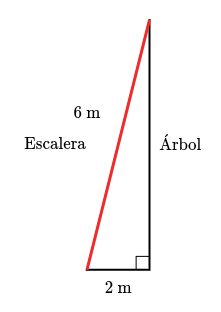
\includegraphics[width=0.2\linewidth]{../images/proverb_pitagoras_06.png}
    \end{center}
    \caption{}
    \label{fig:proverb_pitagoras_06}
\end{figure}

\textbf{¿Qué tan alto en el árbol llegará la escalera?}\\
\textit{Redondea tu respuesta a la décima de metro más cercana.}

\begin{solutionbox}{10cm}
    Podemos usar el teorema de Pitágoras para obtener $x$.
    La ecuación del teorema de Pitágoras es:
    \[c^2=a^2+b^2\]
    donde $a$ y $b$ son las longitudes de los dos catetos del triángulo y $c$ es la longitud de la hipotenusa.
    En este caso, $a=2$, $b=x$ y $c=6$.
    \begin{align*}
        6^2       & =2^2+x^2  \\
        36        & = 4 + x^2 \\
        36-4      & =x^2      \\
        32        & =x^2      \\
        \sqrt{32} & =x        \\
        5.7       & \sim x    \\
    \end{align*}
    La escalera llegará a aproximadamente 5.7 metros en el árbol.
\end{solutionbox}